%-----------------------------------------------
% Template para criação de resumos de projectos/dissertação
% jlopes AT fe.up.pt,   Fri Jul  3 11:08:59 2009
%-----------------------------------------------

\documentclass[9pt,a4paper]{extarticle}

%% English version: comment first, uncomment second
\usepackage[portuguese]{babel}  % Portuguese
%\usepackage[english]{babel}     % English
\usepackage{graphicx}           % images .png or .pdf w/ pdflatex OR .eps w/ latex
\usepackage{times}              % use Times type-1 fonts
\usepackage[utf8]{inputenc}     % 8 bits using UTF-8
\usepackage{url}                % URLs
\usepackage{multicol}           % twocolumn, etc
\usepackage{float}              % improve figures & tables floating
\usepackage[tableposition=top]{caption} % captions
%% English version: comment first (maybe)
\usepackage{indentfirst}        % portuguese standard for paragraphs
%\usepackage{parskip}

%% page layout
\usepackage[a4paper,margin=30mm,noheadfoot]{geometry}

\usepackage{multirow}

%% space between columns
\columnsep 12mm

%% headers & footers
\pagestyle{empty}

%% figure & table caption
\captionsetup{figurename=Fig.,tablename=Tab.,labelsep=endash,font=bf,skip=.5\baselineskip}

%% heading
\makeatletter
\renewcommand*{\@seccntformat}[1]{%
  \csname the#1\endcsname.\quad
}
\makeatother

%% avoid widows and orphans
\clubpenalty=300
\widowpenalty=300

\begin{document}

\title{\vspace*{-8mm}\textbf{\textsc{Estudo, conceção, desenvolvimento e teste de uma aplicação móvel de pagamento e validação para Transportes Públicos de Passageiros}}}
\author{\emph{André Gonçalves Dias}\\[2mm]
\small{Projeto/Dissertação realizado sob a orientação do \emph{Prof.\ João Bernardo de Sena Esteves Falcão e Cunha} e \emph{Dra.\ Marta Maria Campos Ferreira}}}
\date{}
\maketitle
%no page number 
\thispagestyle{empty}

\vspace*{-4mm}\noindent\rule{\textwidth}{0.4pt}\vspace*{4mm}

\begin{multicols}{2}

\section{Motivação}\label{sec:motiva}

Este projeto pretende facilitar os pagamentos e a validação de títulos de viagem nos transportes públicos na Área Metropolitana do Porto, tirando partido de dispositivos móveis. Por outro lado, pretende solucionar o problema causado pelo esquecimento, perda ou extravio de bilhetes, o que muitas vezes leva à necessidade da compra de um novo bilhete e títulos de viagem e, no caso da perda ou extravio, à impossibilidade de utilização dos títulos armazenados no bilhete perdido/extraviado.
\\A principal motivação deste trabalho é o elevado número de passageiros que utilizam os transportes públicos na Área Metropolitana do Porto. Durante o ano de 2012, cinquenta e quatro milhões e meio de passageiros utilizaram o Metro do Porto \cite{INE20130528} e quarenta e cinco milhões de passageiros viajaram nos autocarros da STCP (dados relativos a validações do sistema intermodal) durante o primeiro semestre de 2012. \cite{andante} Outros fatores de motivação são a criação de mobilidade sustentada, facilitar o dia-a-dia dos utilizadores de transportes públicos e, no limite, fomentar uma maior utilização destes transportes na Área Metropolitana do Porto.
\\Se o elevado número de passageiros serviu de base para a escolha da área de desenvolvimento, a escolha do meio tecnológico baseia-se no facto de que atualmente já uma em cada cinco pessoas acede à Internet no telemóvel \cite{INE20121106}, e também de cada vez mais ser menos provável deixar o telemóvel em casa. Um estudo efetuado revela que é mais provável as pessoas saírem de casa sem a carteira do que sem o telemóvel. \cite{NFCForum2011}.
\\Poder adicionar valor aos serviços já existentes é também uma motivação para o desenvolvimento do projeto.

\section{Objetivos}\label{sec:goals}

Os objetivos deste projeto são os seguintes:
\begin{itemize}
\item Criar uma nova forma de pagamento e validação de títulos de viagem, não substituindo os modelos atuais, servindo como um complemento dos mesmos;
\item Reduzir filas nas lojas Andante e postos de venda automáticos, descentralizando a operação de compra de títulos de viagem que muitas vezes causa longos períodos de espera, principalmente no início de cada mês, com a necessidade de renovação das assinaturas;
\item Reduzir custos de emissão e manuseamento de cartões, pois deixa de haver necessidade de um cartão físico, tudo está armazenado no dispositivo móvel do passageiro;
\item Fornecer informação estatística sobre os passageiros aos operadores de transportes, permitindo um melhor ajuste e planeamento de rotas e distribuição de veículos;
\item Possibilitar a realização de múltiplas operações em qualquer lugar e através do um único canal, concentrando um conjunto de serviços à distância de um clique, deixando de haver necessidade de consultar informações nos painéis informativos, comprar títulos de viagem num posto de venda automático ou num balcão e validar o título nas máquinas específicas para esse efeito;
\item Aumentar a satisfação geral dos utilizadores, trazendo-lhes mais comodidade e fornecendo-lhes um serviço que lhes permitirá poupar tempo e trabalho.
\end{itemize}


\section{Descrição do Trabalho}\label{sec:work}

O objetivo deste projeto é remover a necessidade de um elemento físico (cartão) nos pagamentos e validações em transportes públicos na Área Metropolitana do Porto, com a implementação de um sistema de pagamento e validação remoto via Internet, utilizando dispositivos móveis com o sistema operativo Android. Para além disso pretende-se recolher informação relativa às infraestruturas mais utilizadas neste âmbito, estudar as principais funcionalidades e operações existentes para implementação na aplicação e desenvolver soluções apropriadas para os problemas existentes.
\\Como principais requisitos funcionais, este sistema dispõe de funcionalidades de carregamento da carteira virtual, compra e validação (entrada e saída (opcional)) de títulos de viagem, verificação da validade por parte do revisor; sendo estas as necessidades de um sistema tradicional de transportes públicos.\cite{Buttyan2009}
\\Pretende-se que o projeto permita, numa fase posterior, uma integração com a aplicação MOVE-ME já existente no mercado, servindo como uma implementação de funcionalidades extra da mesma e também que seja possível por parte do administrador, a recolha, processamento e análise de informações relativas às viagens dos utilizadores.

\subsection{Arquitetura}

O sistema é composto por três componentes fundamentais. A componente servidor (\emph{Server}) que pode ser considerado o centro do sistema, uma vez que é este que disponibiliza os vários serviços, com a qual as outras componentes interagem remotamente. A componente cliente (\emph{Client}), a qual permite ao passageiro interagir diretamente com os serviços disponibilizados. Finalmente, a componente revisor (\emph{Conductor}), a qual permite aos revisores fiscalizar os passageiros que usam este sistema. De referir que, nesta fase, estas duas últimas componentes estão integradas na mesma aplicação, no telemóvel do passageiro, removendo a necessidade de os revisores andarem equipados com dispositivos apropriados.
\\Esta arquitetura segue a típica arquitetura cliente/servidor. Ver Figura~\ref{fig:architecture}.

\begin{figure}[H]
\centerline{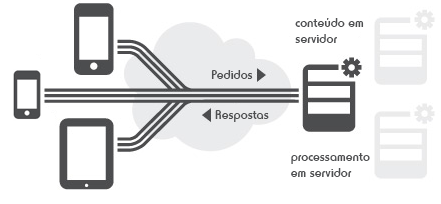
\includegraphics[scale=0.45]{architecture}}
    \caption{Arquitetura Servidor-Cliente}
    \label{fig:architecture}
\end{figure}

\subsection{Android}

A escolha relativa ao sistema operativo recaiu sobre o Android por ser a plataforma móvel mais popular no mundo. Com um dispositivo Android, os utilizadores podem usar todos os serviços Google a que estão habituados, para além de mais de 600 mil aplicações e jogos disponíveis na loja virtual Google Play, sendo que muitas das aplicações são gratuitas. Para além disso, é possível obter milhões de músicas e livros e também milhares de filmes. Os dispositivos Android são melhorados constantemente com lançamentos de atualizações e novas funcionalidades com bastante frequência. Proporcionam também aos utilizadores uma experiência única e personalização de conteúdos.
\\Uma mais valia é o facto de a aplicação MOVE-ME se encontrar também desenvolvida para este sistema operativo, sendo assim mais fácil a integração.
\\A versão base escolhida será 2.2 (Froyo), pois mais de 98\% dos dispositivos possuem esta versão ou superior e ela oferece as funcionalidades necessárias. \cite{dashboards}

\section{Conclusões}\label{sec:conclui}

O facto de cada vez mais utilizadores dos transportes públicos serem possuidores de dispositivos móveis, consumindo informação constantemente, abre as portas à bilhética móvel, não havendo quaisquer entraves por parte do utilizador, que se mostra bastante satisfeito com a comodidade e simplicidade presentes no conceito.
\\Uma outra vantagem deste sistema face a outros na mesma área, é a remoção de quaisquer intervenientes físicos durante todo o processo de utilização. Todas as operações são realizadas através dos dispositivos móveis. No entanto, este sistema tira proveito de um modelo de transportes sem barreiras, como é o caso da Área Metropolitana do Porto, não sendo possível implementá-lo em sistemas fechados sem as devidas modificações que permitissem comunicar com os sistemas de barreiras.

~\\Numa conclusão geral, o conceito está aprovado, é viável e é agora necessário torná-lo robusto e simples de modo a que possa ser utilizado por todos os operadores de transportes públicos da Área Metropolitana do Porto, trazendo-lhes informações adicionais sobre os seus passageiros e também fornecendo aos utilizadores uma solução prática, cómoda e eficaz para as suas deslocações.


%%English version: comment first, uncomment second
\bibliographystyle{unsrt-pt}  % numeric, unsorted refs
%\bibliographystyle{unsrt}  % numeric, unsorted refs
\bibliography{refs}

\end{multicols}

\end{document}
